\documentclass{article}
\usepackage{geometry}
\usepackage{xcolor}
\usepackage{graphicx}
\usepackage{float,lscape}
\usepackage{listings}
\usepackage{color}
\usepackage{lipsum}% Used for dummy text.
\definecolor{titlepagecolor}{cmyk}{1,.60,0,.40}
\definecolor{namecolor}{cmyk}{1,.50,0,.10}
\definecolor{dkgreen}{rgb}{0,0.6,0}
\definecolor{gray}{rgb}{0.5,0.5,0.5}
\definecolor{mauve}{rgb}{0.58,0,0.82}
\lstset{frame=tb,
  language=Java,
  aboveskip=3mm,
  belowskip=3mm,
  showstringspaces=false,
  columns=flexible,
  basicstyle={\small\ttfamily},
  numbers=none,
  numberstyle=\tiny\color{gray},
  keywordstyle=\color{blue},
  commentstyle=\color{dkgreen},
  stringstyle=\color{mauve},
  breaklines=true,
  breakatwhitespace=true,
  tabsize=3
}
%-----------------------------------------------------------------
\begin{document}
\thispagestyle{plain}
\begin{center}
    \Large
    EFM With Field in 100 Starting With Random and Ground Initial States
    
    \vspace{0.4cm}
    \large
    May 5th, 2016 - June 1st, 2016
    
    \vspace{0.4cm}
    \textbf{Andrew Way}
    
    \vspace{0.9cm}
    \textbf{Overview} \\
    \vspace{5mm}
    The effective field method was used to 3000 iterations to determine the 0 temperature states of 
    the 12x12x12 3D FCC kagome lattice while being subjected to a changing magnetic field along the 100 
    direction. The field was either incremented or decremented in steps of 0.0001. 
    There were 4 cases studied:
    \begin{enumerate}
     \item \textbf{Increasing} magnetic field in the \textbf{100} direction from \textbf{0.00 to 0.05},
     with an initial 
     spin configuration that was a \textbf{ground state} with theta = 0.206275 and phi = 3.11867.
     \item \textbf{Increasing} magnetic field in the \textbf{100} direction from \textbf{0.00 to 0.05},
     with an initial 
     spin configuration that was \textbf{randomly generated}.
     \item \textbf{Decreasing} magnetic field in the \textbf{100} direction from \textbf{0.05 to 0.00},
     with an initial
     spin configuration that was a \textbf{ground state} with theta = 0.206275 and phi = 3.11867.
     \item \textbf{Decreasing} magnetic field in the \textbf{100} direction from \textbf{0.05 to 0.00},
     with an initial
     spin configuration that was \textbf{randomly generated}.
    \end{enumerate}
    Analysis that was performed on the resulting data included the following:
    \begin{itemize}
     \item Plots of magnetization versus field
     \item Plots of energy versus field
     \item Animations of the characteristic 6 spins 
     \item Determination of the number of ``unique'' spins that populate the lattice
     \item Determination of the components of the unique spins
     \item Dot products of each of the 6 spins with their respective $``neighbors''$.  
    \end{itemize}

\end{center}
\pagebreak
\thispagestyle{plain}
\begin{center}
\LARGE
RUN 1: Increasing Field, Ground State
\end{center}
\paragraph
\large
Two inflection points are observed in the magnetization graph. There are two inflection points in the
energy graph as well, however they are not as obvious. A planar state is achieved at 0.0041. Between 0.0041 and
0.0064, the brown and green spins become closer to one another, as do the red and purple spins. The pink and blue
spins remain fixed. The spins gradually align with the field, until it suddenly snaps into its final position where
the blue and pink spins point in the same direction, in addition to lying within the xy plane. 
\begin{figure}[h]
 \centering 
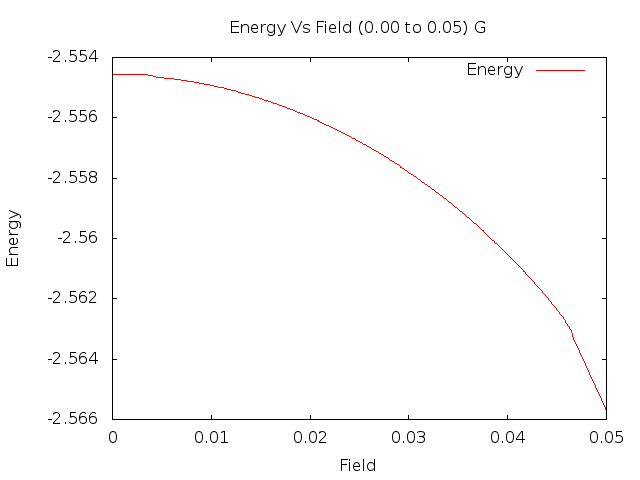
\includegraphics[scale=0.3]{E000to005G.png}
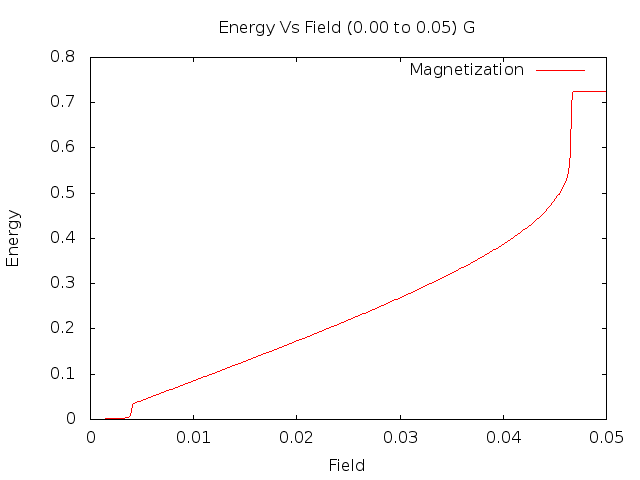
\includegraphics[scale=0.3]{M000to005G.png}
\caption{Energy vs increasing field and Magnetization versus increasing field}
\end{figure}
\begin{figure}[ht]
\centering
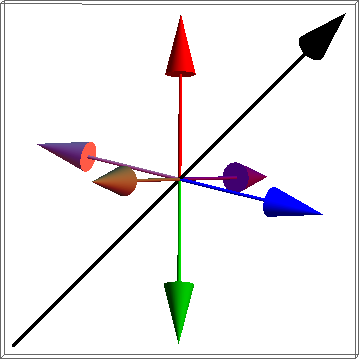
\includegraphics[scale=0.27]{001S000to005G.png}
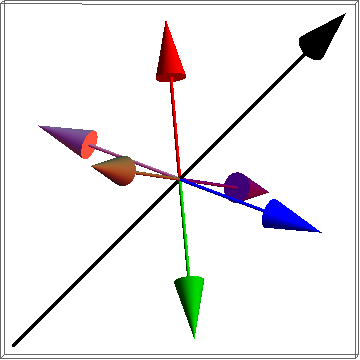
\includegraphics[scale=0.27]{041S000to005G.png}
\includegraphics[scale=0.27]{064S000to005G.png}
\includegraphics[scale=0.27]{455S000to005G.png}
\includegraphics[scale=0.27]{471S000to005G.png}
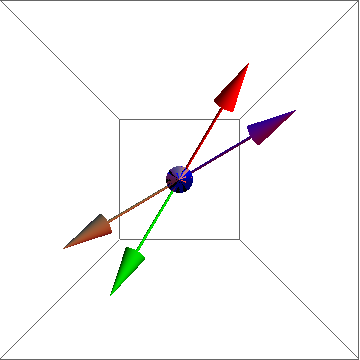
\includegraphics[scale=0.27]{501S000to005G.png}
\caption{H=0, 0.0041, 0.0064, 0.0455, 0.0471, and 0.05}
\end{figure}

\begin{center}
\begin{figure}
\centering
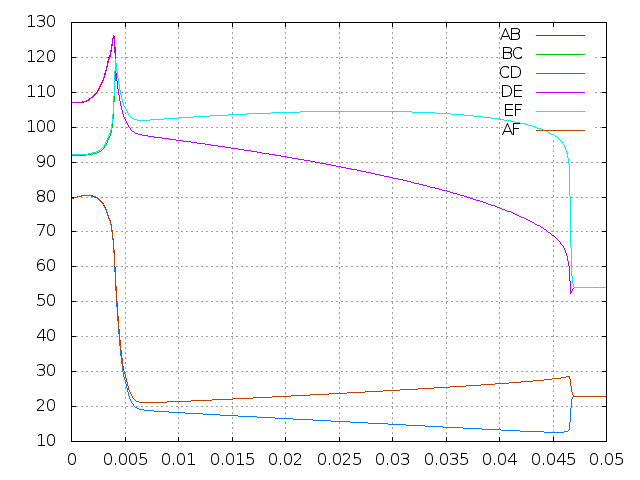
\includegraphics[scale=0.5]{000to005dots.png}
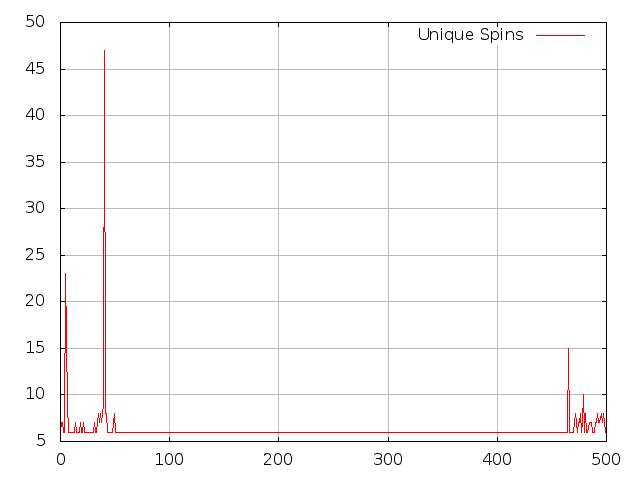
\includegraphics[scale=0.5]{000to005Freq.png}
\caption{Dot products of each spin with its $``neighbour''$. The number of unique spins within the lattice is also present.}
\end{figure}
\end{center}
\pagebreak

\thispagestyle{plain}
\begin{center}
\LARGE
RUN 2: Decreasing Field, Ground State
\end{center}
\paragraph
\large
The initial configuration of the lattice is the same configuration as the final configuration when increasing the field.
See Run 1. As the field is decreased, the spins are released from the nonplanar state, and return to the typically observed
planar state, that gradually unaligns with the field direction as the field is decreased. Finally, the spins return
to a full planar state. 
\begin{figure}[ht]
 \centering 
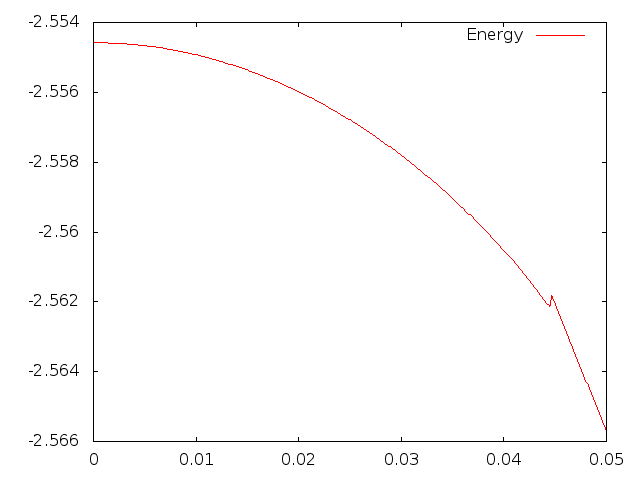
\includegraphics[scale=0.3]{E005to000G.png}
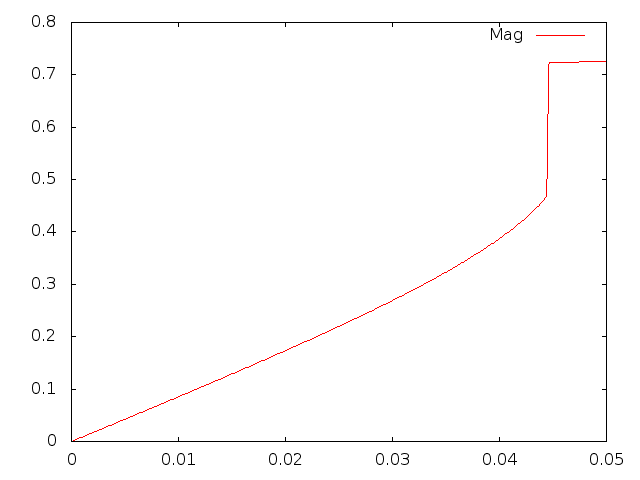
\includegraphics[scale=0.3]{M005to000G.png}
\caption{Energy vs decreasing field and Magnetization versus decreasing field}
\end{figure}
\begin{figure}[ht]
\centering
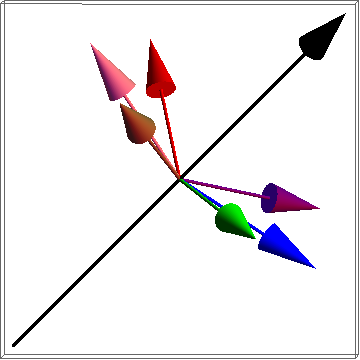
\includegraphics[scale=0.27]{001S005to000G.png}
\includegraphics[scale=0.27]{54S005to000G.png}
\includegraphics[scale=0.27]{055S005to000G.png}
\includegraphics[scale=0.27]{056S005to000G.png}
\includegraphics[scale=0.27]{255S005to000G.png}
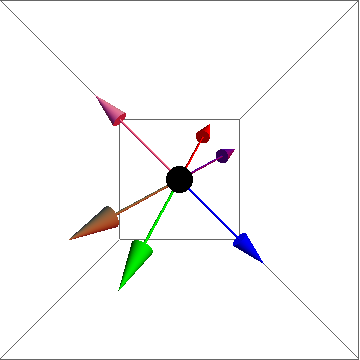
\includegraphics[scale=0.27]{501S005to000G.png}
\caption{H=0.05, 0.0447, 0.0446, 0.0445, 0.0244, and 0}
\end{figure}

\begin{figure}
\centering
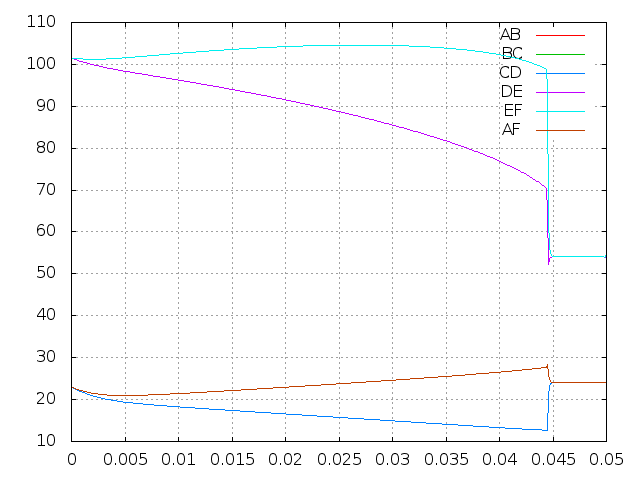
\includegraphics[scale=0.5]{005to000dots.png}
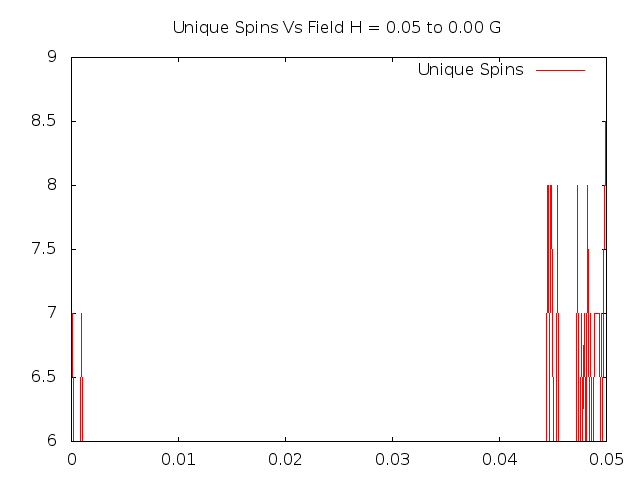
\includegraphics[scale=0.5]{005to000Freq.png}
\caption{Dot products of each spin with its neighbours. The X-axis has been incorrectly factored
by 1/10 in the dot product graph. The number of unique spins within the lattice is also present.}
\end{figure}

\pagebreak 

\thispagestyle{plain}
\begin{center}
\LARGE
RUN 3: Increasing Field, Random State
\end{center}
\paragraph
\large
The energy drops very quickly at near zero field, which is likely because of insufficient number of iterations. Two
points of inflection are observed, as in Run 1. The transition of the spins is very similar to starting from a ground
state.}
\begin{figure}[h]
 \centering 
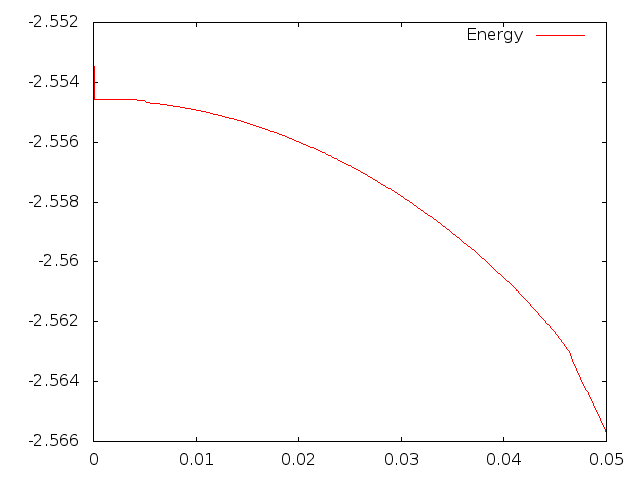
\includegraphics[scale=0.3]{E000to005R.png}
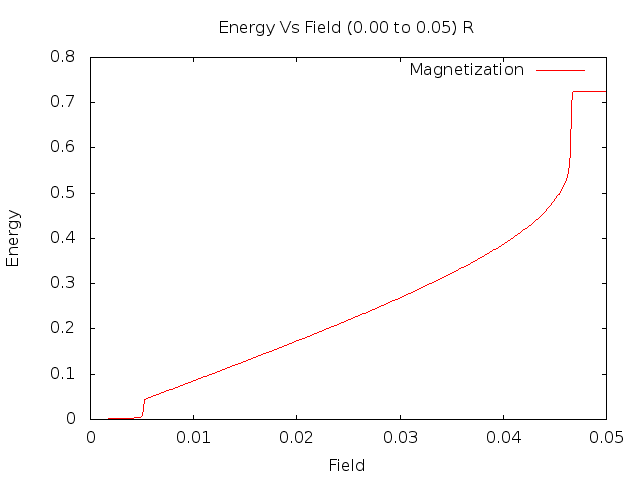
\includegraphics[scale=0.3]{M000to005R.png}
\caption{Energy vs increasing field and Magnetization versus increasing field}
\end{figure}
\begin{figure}[ht]
\centering
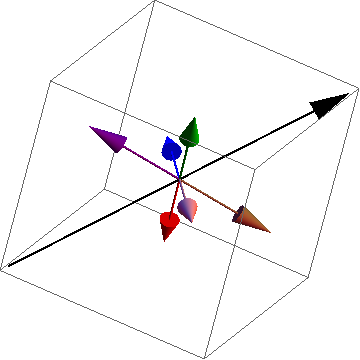
\includegraphics[scale=0.22]{001S000to005R.png}
\includegraphics[scale=0.22]{002S000to005R.png}
\includegraphics[scale=0.22]{047S000to005R.png}
\includegraphics[scale=0.22]{052S000to005R.png}
\includegraphics[scale=0.22]{054S000to005R.png}
\includegraphics[scale=0.22]{057S000to005R.png}
\includegraphics[scale=0.22]{067S000to005R.png}
\includegraphics[scale=0.22]{430S000to005R.png}
\includegraphics[scale=0.22]{466S000to005R.png}
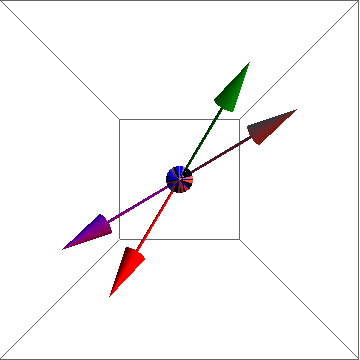
\includegraphics[scale=0.22]{501S000to005R.png}
\caption{H = 0.00, 0.0002, 0.0047, 0.0052, 0.0054, 0.0057, 0.067, 0.0430, 0.0466, 0.05}
\end{figure}

\begin{center}
\begin{figure}
\centering
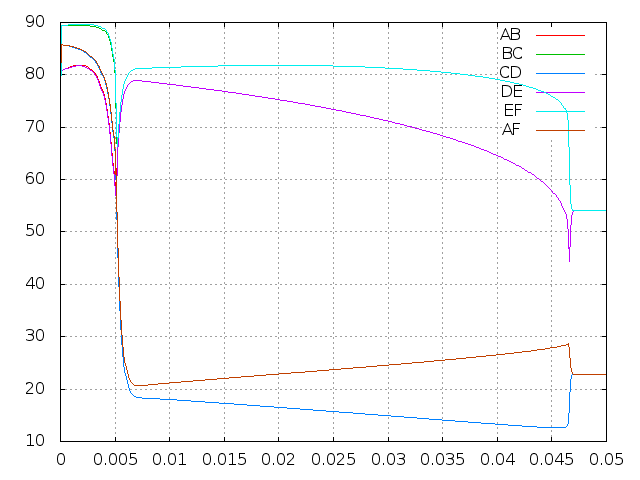
\includegraphics[scale=0.5]{000to005Rdots.png}
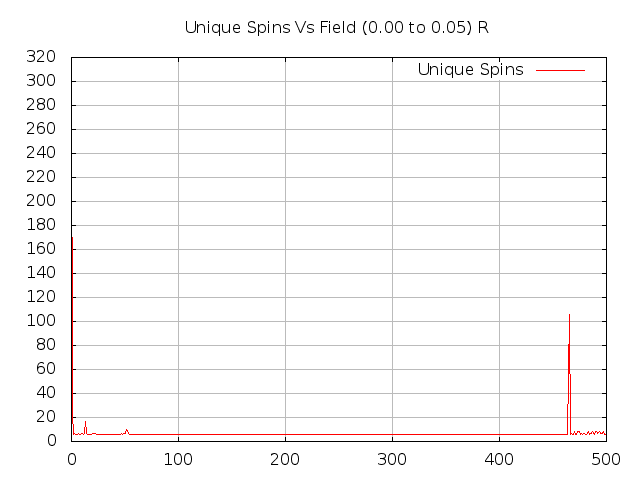
\includegraphics[scale=0.5]{000to005RFreq.png}
\caption{Dot products of each spin with its ``neighbour''. The X-axis has been incorrectly factored
by 1/10in the dot product graph. The number of unique spins within the lattice is also present.}
\end{figure}
\end{center}
\pagebreak

\thispagestyle{plain}
\begin{center}
\LARGE
RUN 4: Decreasing Field, Random State
\end{center}
\paragraph
\large
The lattice starts off in a planar state. As the field is decreased, spins gradually unalign with the field. 
Suddenly, at 0.0455, the spins snap back into a slight realigned planar state. Another sudden readjustment
is observed at 0.025. Finally, the spins return a full planar state at 0 field. The red and brown spins
swap positions as the field lowers, as do the green and purple spins. 
\begin{figure}[h]
 \centering 
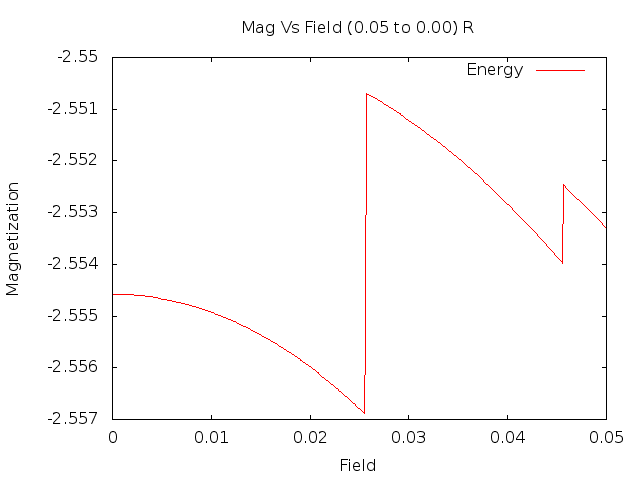
\includegraphics[scale=0.3]{E005to000R.png}
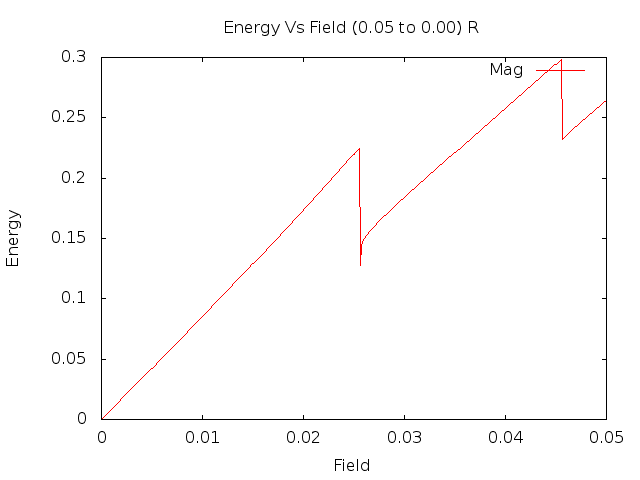
\includegraphics[scale=0.3]{M005to000R.png}
\caption{Energy vs decreasing field and Magnetization versus decreasing field}
\end{figure}
\begin{figure}[ht]
\centering
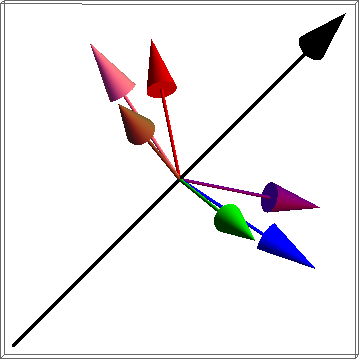
\includegraphics[scale=0.23]{001S005to000R.png}
\includegraphics[scale=0.23]{044S005to000R.png}
\includegraphics[scale=0.23]{046S005to000R.png}
\includegraphics[scale=0.23]{243S005to000R.png}
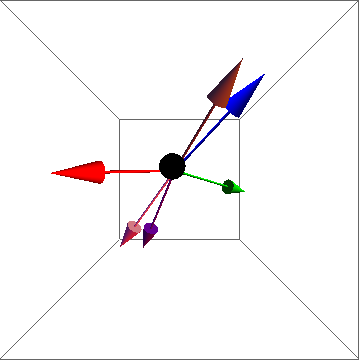
\includegraphics[scale=0.23]{245S005to000R.png}
\includegraphics[scale=0.23]{246S005to000R.png}
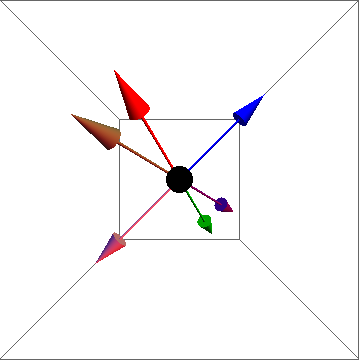
\includegraphics[scale=0.23]{501S005to000R.png}
\caption{H = 0.05, 0.0457, 0.0455, 0.0258, 0.0256, 0.0255, 0.00.}
\end{figure}

\begin{figure}
\centering
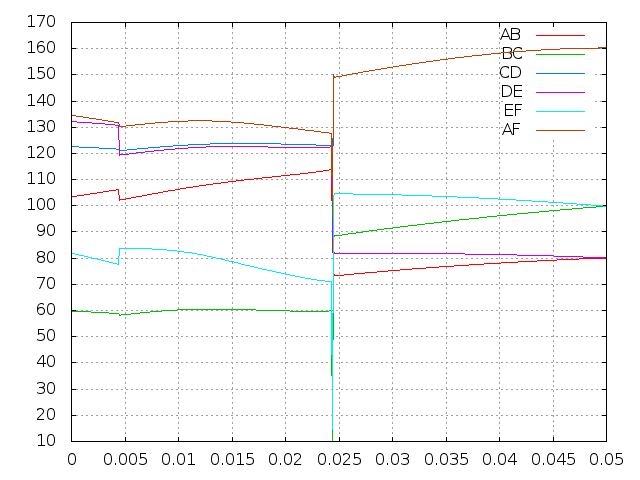
\includegraphics[scale=0.5]{005to000Rdots.png}
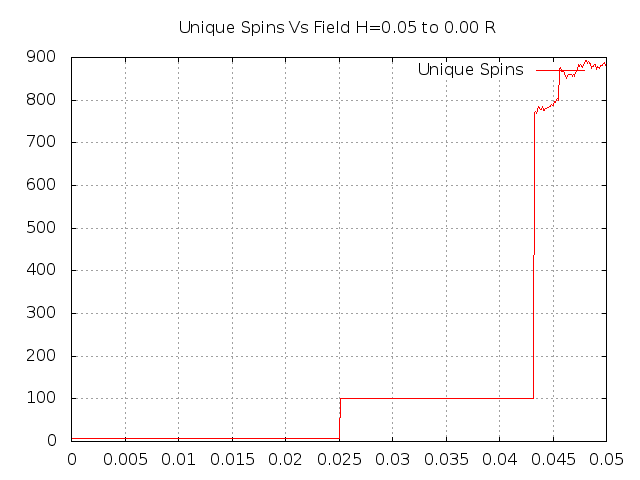
\includegraphics[scale=0.5]{005to000RFreq.png}
\caption{At high field, a huge number of $``unique''$ spins was observed. When looking through one of the configuration
files, most spins only agreed with some other spins to at most 1 decimal place. The program that determines whether
a spin is unique considers a spin to be unique when it doesn't agree with any previously found spin up to at least two decimal 
places. Hence, the large number of unique spins present.The plateau in the middle is actually just false data I put
into the text file, since I cancelled the program since it was taking a very long time. I reran the program from around
H = 0.0250 to 0, and found that the lattice in this field range always had 6 unique spins.}
\end{figure}

\end{document}